% !TeX TXS-program:compile = txs:///lualatex | txs:///view
\documentclass[11pt]{beamer}
\usepackage[spanish]{babel}
\usetheme{Boadilla}
\author[Carlos Aznarán]{Carlos Alonso Aznarán Laos}
\title{Presentación}
\setbeamercovered{transparent}
\setbeamertemplate{navigation symbols}{}
\logo{UNMSM1}
\institute[UNI]{Universidad Nacional de Ingeniería}
\date{\today}
\subject{}
\begin{document}

\begin{frame} % título de contenidos
	\titlepage
\end{frame}

\begin{frame}
	\tableofcontents % es importante
\end{frame}

\section{El problema}

\begin{frame}{El problema de investigación}
	Existe xxx, sin embargo yyy.
\end{frame}

\begin{frame}{Objetivo}
	Diseñar un plan de seguridad. %Verbos en infinitivo
\end{frame}

\begin{frame}{Resultados}
	\centering
	
\includegraphics[scale=0.6]{boxplot}
\end{frame}

\begin{frame}{Resultados}
	\centering
	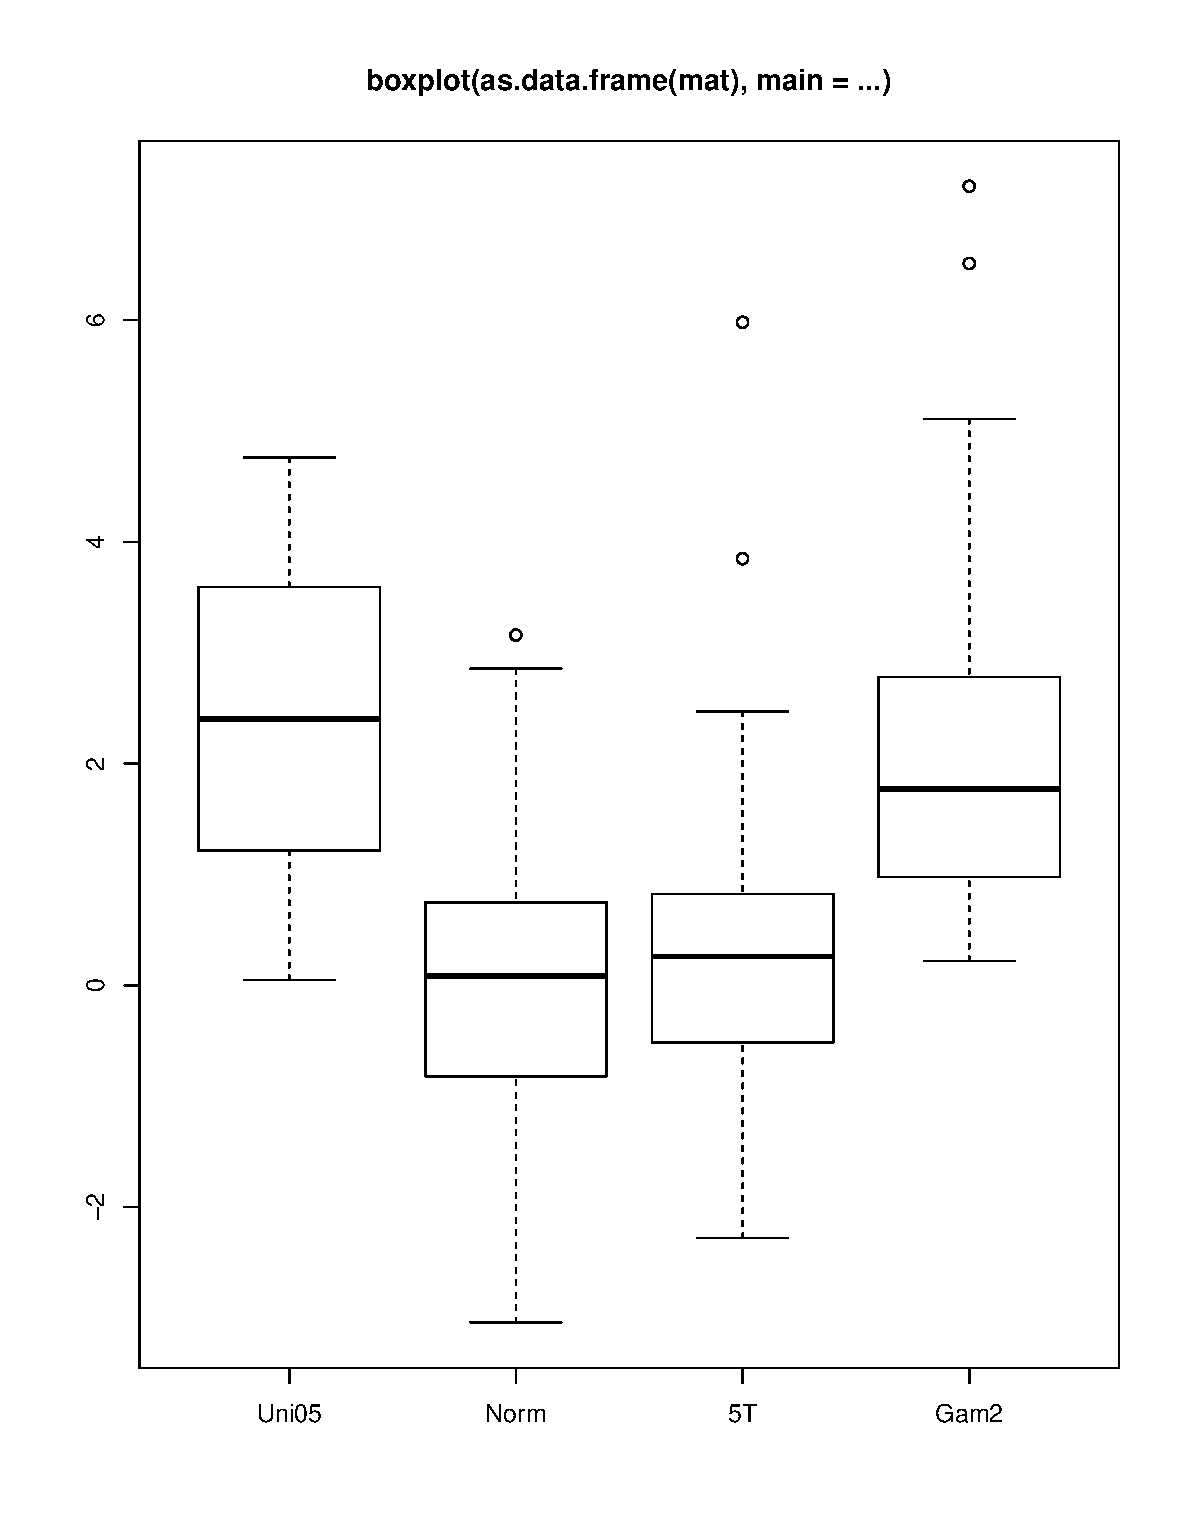
\includegraphics[scale=0.31]{b}
\end{frame}
\end{document}
